\documentclass{article}
\usepackage{tikz}

\begin{document}

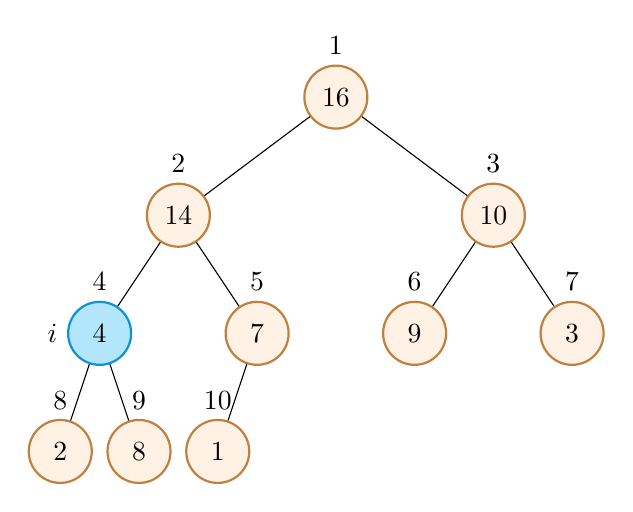
\begin{tikzpicture}[
level distance=1.5cm,
level 1/.style={sibling distance=4cm},
level 2/.style={sibling distance=2cm},
level 3/.style={sibling distance=1cm},
normal/.style={circle,draw=brown,fill=orange!10,thick,minimum size=8mm},
active/.style={circle,draw=cyan!80!blue,fill=cyan!30,thick,minimum size=8mm}
]

\node[normal,label=above:1]{16}
child{
    node[normal,label=above:2]{14}
    child{
        node[active,label=above:4,label=left:$i$]{4}
        child{node[normal,label=above:8]{2}}
        child{node[normal,label=above:9]{8}}
    }
    child{
        node[normal,label=above:5]{7}
        child{node[normal,label=above:10]{1}}
        child[missing]
    }
}
child{
    node[normal,label=above:3]{10}
    child{node[normal,label=above:6]{9}}
    child{node[normal,label=above:7]{3}}
};

\end{tikzpicture}

\end{document}
